\chapter{Ventilation Plant}
\label{chp:ventilationPlant}
\fancyhead[C]{Chapter \ref{chp:ventilationPlant}}

\section{\gls{AHU} Components}
\label{sec:AHUComponents}

\begin{figure}[H]
\centering
\begin{tikzpicture}[scale=0.8, every node/.style={scale=0.8}]

%AHU Casing and labels
\draw [black] (2.5,0) rectangle (15,4);
\draw [gray] (2.5,2) -- (15,2);

\draw [<-] (0,1) -- (2,1);
\draw [->] (0,3) -- (2,3);

\node [above] at (1,3) {Air Intake};
\node [above] at (1,1) {Exhaust Air};

\draw [->] (15.5,1) -- (17.5,1);
\draw [<-] (15.5,3) -- (17.5,3);

\node [above] at (16.5,3) {Return Air};
\node [above] at (16.5,1) {Supply Air};

%Intake & Exhaust Dampers

\draw [gray] (2.5,2) rectangle (3,4);
\draw [gray] (2.5,0) rectangle (3,2);

\draw [gray] (2.5,4) -- (3,3.5) -- (2.5,3) -- (3,2.5) -- (2.5,2);
\draw [fill, gray] (2.75,3.75) circle [radius=0.05];
\draw [fill, gray] (2.75,3.25) circle [radius=0.05];
\draw [fill, gray] (2.75,2.75) circle [radius=0.05];
\draw [fill, gray] (2.75,2.25) circle [radius=0.05];

\draw [gray] (2.5,0) -- (3,0.5) -- (2.5,1) -- (3,1.5) -- (2.5,2);
\draw [fill, gray] (2.75,1.75) circle [radius=0.05];
\draw [fill, gray] (2.75,1.25) circle [radius=0.05];
\draw [fill, gray] (2.75,0.75) circle [radius=0.05];
\draw [fill, gray] (2.75,0.25) circle [radius=0.05];

\node [above] at (2.75,4) {(1)};
\node [below] at (2.75,0) {(11)};

%Frost Coil

\draw [gray] (3.25,4.1) -- (3.25,2.1) -- (3.35,2.1) -- (3.35,3.9) -- (3.45,3.9) -- (3.45,2.1) -- (3.55,2.1) -- (3.55,4.1);

\node [above] at (3.4,4) {(2)};

%Supply Filters (Panel and then Box)

\draw [gray] (4,2) rectangle (4.5,4);
\draw [gray] (4.5,2) rectangle (5.75,4);

\draw [gray] (4,2) -- (4.5,2.5) -- (4,3) -- (4.5,3.5) -- (4,4);
\draw [gray, rounded corners] (4.5,2) -- (5.65,2.3) -- (5.65,2.7) -- (4.5,3) -- (5.65,3.3) -- (5.65,3.7) -- (4.5,4);

\node [above] at (4.25,4) {(3)};
\node [above] at (5.125,4) {(4)};

%PHX Drawing

\draw [gray] (6,0) rectangle (10,4);
\draw [gray] (8,0) -- (10,2) -- (8,4) -- (6,2) -- (8,0);
\node [above] at (8,4) {(5)};

%Supply Fan

\draw [gray] (10.25,0) rectangle (12.25,2);
\fill [gray, pattern= north west lines, opacity=0.4,draw] (11.25,1) circle [radius = 0.75];
\fill [gray, fill = white, opacity=1, draw] (11.25,1) circle [radius = 0.4];
\draw [fill, gray] (11.25,1) circle [radius=0.1];
\draw [gray] (10.75,0) -- (11.25,1) -- (11.75,0);
\node [below] at (11.25,0) {(6)};

%Cooling Coil

\draw [gray] (12.5,-0.1) -- (12.5,1.9) -- (12.6,1.9) -- (12.6,0.1) -- (12.7,0.1) -- (12.7,1.9) -- (12.8,1.9) -- (12.8,0.1) -- (12.9,0.1) -- (12.9,1.9) -- (13,1.9) -- (13,0.1) -- (13.1,0.1) -- (13.1,1.9) -- (13.2,1.9) -- (13.2,0.1) -- (13.3,0.1) -- (13.3,1.9) -- (13.4,1.9) -- (13.4,-0.1);

\node [below] at (12.95,0) {(7)};

%Re-heat Coil

\draw [gray] (14,-0.1) -- (14,1.9) -- (14.1,1.9) -- (14.1,0.1) -- (14.2,0.1) -- (14.2,1.9) -- (14.3,1.9) -- (14.3,0.1) -- (14.4,0.1) -- (14.4,1.9) -- (14.5,1.9) -- (14.5,-0.1);

\node [below] at (14.25,0) {(8)};

%Return Air Filter (Panel)

\draw [gray] (10.25,2) rectangle (10.75,4);
\draw [gray] (10.75,4) -- (10.25,3.5) -- (10.75,3) -- (10.25,2.5) -- (10.75,2);
\node [above] at (10.5,4) {(9)};

%Return Air Fan

\draw [gray] (5.75,0) rectangle (3.75,2);
\fill [gray, pattern= north west lines, opacity=0.4,draw] (4.75,1) circle [radius = 0.75];
\fill [gray, fill = white, opacity=1, draw] (4.75,1) circle [radius = 0.4];
\draw [fill, gray] (4.75,1) circle [radius=0.1];
\draw [gray] (4.25,0) -- (4.75,1) -- (5.25,0);
\node [below] at (4.75,0) {(10)};

\end{tikzpicture}
\caption{Typical \gls{AHU} schematic, the component numbering follows the air path from outdoor air (Air Intake) through to the space (Supply Air), and then from the return air back to exhaust air.}
\label{fig:TypicalAHUSchematic}
\end{figure}

A typical \gls{AHU} schematic is shown in figure~\ref{fig:TypicalAHUSchematic}, (1) \& (11) are motorised dampers, (2) is a frost coil, (3) \& (9) are panel filters, (4) is a bag filter, (5) is a counter-flow plate heat exchanger, (6) \& (10) are supply and extract fans respectively, (7) is a cooling coil, (8) is a heating or re-heat coil.

\subsection{Energy Recovery Devices}

A number of heat recovery devices are available for inclusion within an \gls{AHU}.

\begin{itemize}
\item Plate Heat Exchanger,
\item Thermal Wheel,
\item Run-Around-Coil,
\item Mixing Box,
\end{itemize}

\subsubsection{Plate Heat Exchanger}

The plate heat exchanger works by passing the opposing air streams (supply and extract) through fins within the unit and heat transfer occurs through the metal fins without the two air streams coming into contact with each other.  See~\autoref{fig:PHXWithLabels} for a schematic example of a plate heat exchanger in a cross flow configuration.

\subsubsection{Thermal Wheel}

Thermal wheel units utilise a metal perforated wheel which is constantly rotating, this warms up in the extract air stream and then the warm section is rotated into the supply air stream and transfers heat to the air.  Thermal wheels mix small amounts of the air streams, and involves the running of a motor to drive the wheel.

\subsubsection{Run-Around-Coil}

Run-Around-Coil units use two finned coils (similar to the heating and cooling coils) filled with a glycol/water mixture, and run the mixture between the two coils positioned in each of the air streams (supply and extract).  This system utilises a pump, and associated pressurisation equipment in order to pass water/glycol between the two coils.

\subsubsection{Mixing Box}

Mixing Box units recirculate a proportion of the air streams in order to satisfy external air supply and heating/cooling loads simultaneously, for example if the air supply to support the cooling load of a space is double the outdoor air provision, then a mixing box can be used to recirculate half the cooling load air flow rate and allow the rest to come from outside.  This can reduce the amount of conditioning required for the supply air as the recirculated air may be closer to the required set-point than the external air.

\subsubsection{ErP Regulations}

Under the ErP regulations\footnote{Known by many different names: Energy related Products (ErP), Ecodesign Directive (\textnumero~2009/125/EC), Lot 6 - Ventilation Units, Ecodesign Regulation (\textnumero~1253/2014), UK Statutory Instrument 2015 (\textnumero~469)}, some form of energy recovery must be used and only plate heat exchangers, thermal wheels, or run-around-coils are acceptable.  In general the regulations apply to bi-directional and uni-directional ventilation units within commercial sized buildings; however, there are exceptions for certain applications such as Swimming Pools, Agricultural Buildings, Foundries etc.

\subsubsection{\gls{HTM} 03-01 Standard AHU Layout}

\gls{HTM} 03-01 prescribes a standard AHU layout for healthcare applications, this layout includes a plate heat exchanger as the energy recovery device.  The layout includes a fog coil, which is designed to prevent ice build-up on the filters and plate heat exchanger during the winter design condition, which is typically fully saturated air at temperatures lower than \SI{0}{\celsius}.  The layout also includes a cooling coil and a heating coil, which are used to condition the supply air to the required set point.  The cooling coil is positioned before the heating coil to prevent any potential freezing within the coil; however, this precludes the ability to dehumidify the air stream should it be necessary/desired.  The layout also includes a bag filter on the supply air side, and panel filters on the extract air side, this is to prevent any potential damage to the energy recovery device from dirty air, and to ensure that the supply air is clean for the space.

\todo[inline, color=blue!10]{Include a schematic of the HTM 03-01 standard AHU layout, and reference it in the text above. Check layout against the standard, and ensure that the component numbering is consistent with the typical AHU schematic shown in \autoref{fig:TypicalAHUSchematic}.}

\subsection{Energy Recovery Calculations}

\autoref{eq:HREfficiency} shows the equation describing the efficiency of the heat recovery unit ($\eta$) and the temperatures at each point for balanced air flow rates (i.e. supply air flow rate is equal to extract air flow rate), this equation is derived in Derivation \ref{der:PHXEfficiency} and shows allows for unbalanced air streams (i.e. supply air rate does not equal the extract air rate).  \autoref{fig:PHXWithLabels} shows a plate heat exchanger (PHX) and the appropriate labels to correspond to \autoref{eq:HREfficiency}.  Minimum values prescribed in the ErP regulations for heat recovery efficiency can be found in \autoref{tab:HREff}.

\begin{equation}\label{eq:HREfficiency}
\eta = \frac{t_2 - t_1}{t_3 - t_1} = \frac{t_{co} - t_{ci}}{t_{hi} - t_{ci}}
\end{equation}

\begin{figure}
\centering
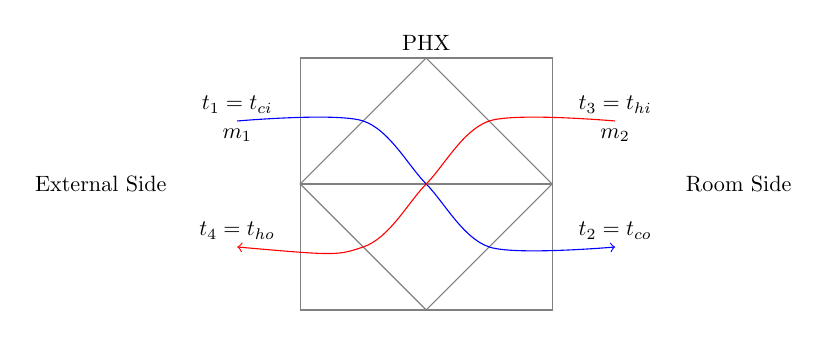
\begin{tikzpicture}[scale=0.8, every node/.style={scale=0.8}]


%PHX Drawing

\draw [gray] (6,0) rectangle (10,4);
\draw [gray] (8,0) -- (10,2) -- (8,4) -- (6,2) -- (8,0);
\draw [gray] (6,2) -- (10,2);
\node [above] at (8,4) {PHX};

\node [right] at (12,2) {Room Side};
\node [left] at (4,2) {External Side};

%Air Path Drawings

\draw [blue, ->] plot [smooth] coordinates {(5,3) (7,3) (8,2) (9,1) (11,1)};
\draw [red, <-] plot [smooth] coordinates {(5,1) (7,1) (8,2) (9,3) (11,3)};

%Node labels

\node [above] at (11,1) {$t_2 = t_{co}$};
\node [above] at (11,3) {$t_3 = t_{hi}$};

\node [above] at (5,1) {$t_4 = t_{ho}$};
\node [above] at (5,3) {$t_1 = t_{ci}$};

\node [below] at (5,3) {$m_1$};
\node [below] at (11,3) {$m_2$};

\end{tikzpicture}
\caption{A counter-flow plate heat exchanger (PHX) showing air flow paths and temperature labels corresponding to \autoref{eq:HREfficiency}.}
\label{fig:PHXWithLabels}
\end{figure}

\begin{table}
\centering
\begin{tabular}{cc}
\hline
Heat Recovery Type & ErP 2018 Minimum Efficiency\\
\hline
Plate Heat Exchanger & 73\%\\
Thermal Wheel & 73\%\\
Run-Around-Coil & 68\%\\
\hline
\end{tabular}
\caption{Table showing the minimum efficiency required for the three acceptable heat recovery equipment types in air handling units}
\label{tab:HREff}
\end{table}


\begin{derivation}
\label{der:PHXEfficiency}
\onehalfspacing

This is a derivation of the energy balance within an AHU heat recovery device allowing for unbalanced air flow rates.  First we start with the basic energy balance equation defined in \autoref{eq:BasicEnergyBalance}.

\[Q = m~C_p~\delta t\]

Now we consider the supply air air-path (Cold), and the extract air air-path (Hot) separately.

\[Q_{cold} = m~C_p~(t_{co} - t_{ci})\]
\[Q_{hot} = m~C_p~(t_{hi} - t_{ho})\]

Using the above energy balances we can calculate the cold out temperature (Supply Air, Room side) if we know the temperature of the other three air streams, as this is rarely the case, we need to make some assumptions

If the heat exchanger were to be infinitely long, then the temperature of the hot in and cold out positions would be equal, i.e.

\[t_{hi} = t_{co}\]

Now in order to know the air temperature leaving the heat exchanger on the supply air side ($t_{co}$), we would only have to know what the extract air temperature is ($t_{hi}$); similarly, the temperature of the hot out ($t_{ho}$) and cold in ($t_{ci}$) positions would be equal, i.e.

\[t_{ho} = t_{ci}\]

An infinitely long heat exchanger is impractical (and impossible), so we can account for the reduction in heat transfer by using an efficiency term ($\eta$) as a ratio of the energy balances, i.e.

\[\frac{Q_{1,cold}}{Q_{2,hot}} = \frac{m_1~C_p~(t_{co} - t_{ci})}{m_2~C_p~(t_{hi} - t_{ho})}\]

let $\eta \times t_{ci} = t_{ho}$

\[\eta = \frac{m_1~\cancel{C_p}~(t_{co} - t_{ci})}{m_2~\cancel{C_p}~(t_{hi} - t_{ci})}\]

using the labels in \autoref{fig:PHXWithLabels}, the equation becomes;

\[\eta = \frac{m_1}{m_2} \frac{t_2 - t_1}{t_3 - t_1}\]

\textbf{\textit{QED}}

\end{derivation}

\subsection{Frost Coils}
\label{ssec:FrostCoils}

During the winter ventilation design condition, which is typically fully saturated air at temperatures lower than \SI{0}{\celsius}, the build-up of ice within an AHU is possible.  Ice can build-up on filters, plate-heat exchangers, or coils that are not heated (i.e. cooling coils or in-active heating coils), but typically only when the unit is running.  To combat the ice build up, frost coils can be installed which are sized with sufficient capacity to raise the temperature from the external design condition (say \SI{-5}{\celsius}) to a positive temperature (typically \SI{5}{\celsius}).

Whilst the unit is operational it is fair to assume that the heating coil and energy recovery devices will be activated and so any damage from ice build up will be limited to the filters (shown at locations (2) and (3) in \autoref{fig:TypicalAHUSchematic}), as the energy recovery device will warm the incoming air using the return air.  When a filter is frozen there is a risk that the filter will break up, or be pulled through the unit by the action of the fans, which will potentially damage the energy recovery device, or downstream filters.  Certain manufacturers will guarantee that their filters can be used in freezing conditions without breaking, therefore negating the need for a frost coil but bringing a component of risk.

Using a frost coil within an AHU will increase the internal static pressure required to be overcome by the fans (Increasing specific fan power (SFP)), reduce the difference in temperature across the energy recovery device (reducing the 'free' energy applied to the supply air stream\footnote{'free' in the sense of recovered energy that would otherwise be lost to atmosphere without the energy recovery device}), and increase the cost of both the unit and installation.

If a frost coil is omitted from an AHU then additional precautions are required, for example, additional control routines would be built into the control system that would shut dampers if the unit begins to freeze and turn the heating coil to full to attempt to defrost any frozen components.  If a cooling coil is present within the unit, then it would need to be sited after the heating coil to prevent any potential freezing within the coil; however, this precludes the ability to dehumidify the air stream should it be necessary/desired.

\subsubsection{Fog Coils}

The concept of a fog coil was introduced by \gls{HTM} 03-01\footnote{HTM 03-01: Specialised ventilation for healthcare premises, Part A: Design and validation, 2018} as an alternative to the standard frost coils described previously in \autoref{ssec:FrostCoils}.  The fog coil is designed to increase the incoming temperature by a fixed amount, typically, \SI{3}{\celsius}, this moves the incoming air condition away from the dew point without the need to raise the temperature to a positive value, and therefore reduces the energy demand of the coil and the associated increase in fan power.

\subsubsection{Calculations with and without Frost Coils}

If we consider two AHU with both with a design volumetric air flow rate of \SI{1}{\cubic\metre\per\second}, a energy recovery device with an efficiency, $\eta$, of 73\%, and one unit with a frost coil and one without, we can compare the difference in running costs.  We are considering the winter time design, so external temperature is \SI{-5}{\celsius}, and the AHU supply temperature set point is 20\si{\celsius}.

Lets consider the LTHW load, \autoref{eq:AHUfrostCoilExample} shows the required LTHW mass flow rate with a frost coil at our design duty, and \autoref{eq:AHUnoFrostCoilExample} shows the required LTHW mass flow rate without a frost coil.

Firstly the AHU with a frost coil, we consider the energy required to heat \SI{1}{\cubic\metre\per\second} of air from \SI{-5}{\celsius} to \SI{5}{\celsius}:

\begin{equation}
Q = 1 \times 1.2 \times 1.005 \times (5--5) = 12.06 kW
\end{equation}

Now with a off coil temperature of \SI{5}{\celsius} from our frost coil and a return air temperature of \SI{20}{\celsius} we can calculate the temperature gain across our energy recovery device (Using \autoref{eq:HREfficiency} described earlier):

\begin{equation}
t_2 = (0.73 \times (20 - 5)) + 5 = 15.95\si{\celsius}, say~16\si{\celsius}
\end{equation}

Finally we need the energy required to heat our air stream from \SI{16}{\celsius} to \SI{20}{\celsius}:

\begin{equation}
Q = 1 \times 1.2 \times 1.005 \times (20-16) = 4.82 kW
\end{equation}

So in total we require $12.06 + 4.82 = 16.88 kW$ of LTHW input, the mass flow rate of which is:

\begin{equation}\label{eq:AHUfrostCoilExample}
m = \frac{16.88}{4.187 \times (80-60)} = 0.20 kg/s
\end{equation}

Now we consider the same AHU without the frost coil, ignoring any detriment to frozen filters etc.  We know that the air stream is at \SI{-5}{\celsius} and our return air is at \SI{20}{\celsius}, so the temperature rise across our energy recovery device is:

\begin{equation}
t_2 = (0.73 \times (20 - -5)) + -5 = 13.25\si{\celsius}, say~13\si{\celsius}
\end{equation}

This is only three degrees lower than our example with a frost coil, meaning that we recover a lot more heat due to the larger temperature difference, raising the temperature \SI{18}{\celsius} compared to \SI{6}{\celsius} with a frost coil.  Now we need to calculate the required energy to heat our air stream from \SI{13}{\celsius} to \SI{20}{\celsius}:

\begin{equation}
Q = 1 \times 1.2 \times 1.005 \times (20-13) = 8.44 kW
\end{equation}

The LTHW input to this unit is:

\begin{equation}\label{eq:AHUnoFrostCoilExample}
m = \frac{8.44}{4.187 \times (80-60)} = 0.10 kg/s
\end{equation}

This difference in LTHW mass flow rate is vast, and when considering LTHW generation via natural gas boilers (assuming 90\% efficiency) the running cost is as below:

Firstly the unit with frost coils:

\begin{equation}
0.20 / 0.9 = 0.22 kg/s
\end{equation}

\begin{equation}
Q = 0.22 \times 4.187 \times (80-60) = 18.42 kW
\end{equation}

And assuming a cost of \SI{2.57}{p\per\kilo\watt\hour}, the LTHW required by the AHU with frost coils costs £11.36 per 24 hours when the external temperature is \SI{-5}{\celsius}.  The AHU without frost coils:

\begin{equation}
0.10 / 0.9 = 0.11 kg/s
\end{equation}

\begin{equation}
Q = 0.11 \times 4.187 \times (80-60) = 9.21 kW
\end{equation}

Using the costs above, the LTHW generation for the AHU without frost coils costs £5.68 per 24 hours.  Although the cost is relatively small this is the cost of generating LTHW to serve the AHU demand, and the  difference can add up when considering the complete winter period where temperatures can be negative for a lot longer than 24 hours!  This cost analysis does not consider the increase in fan running cost due to the increased resistance from the frost coil, which affects the running cost year-round whether the frost coil is active or not.  \autoref{tab:FrostCoilCost} give a summary of the running energy and costs for an AHU with and without a frost coil, a fog coil has also been included in the table for comparison.

\begin{table}
\centering
\begin{tabular}{cccc}
\hline
Pre-Coil Type & HR Temperature (ho) & Heating Demand & Cost per 24 hours\\
\hline
Frost & \SI{16}{\celsius} & \SI{0.20}{\kilo\gram\per\second} & \pounds11.36 \\
Fog & \SI{14}{\celsius} & \SI{0.13}{\kilo\gram\per\second} & \pounds7.43 \\
None & \SI{13}{\celsius} & \SI{0.10}{\kilo\gram\per\second} & \pounds5.68 \\
\hline
\end{tabular}
\caption{Table showing differences in AHU running costs both with and without a frost coil.  The AHU considered has a flow rate of \SI{1}{\cubic\metre\per\second}, a energy recovery device with an efficiency of 73\%, and a supply air set point of \SI{20}{\celsius}.  The external air temperature in this example is \SI{-5}{\celsius} and fully saturated.}
\label{tab:FrostCoilCost}
\end{table}

\subsection{Filtration}



\subsection{Fans}



\subsection{Heating/Cooling Coils}



\subsubsection{Dehumidification}



\section{Component Resistance}

\todo[inline, color=blue!10]{Filter Resistance dirty/average/clean etc., coil resistance, PHX vs thermal wheel resistance}


\section{Fan Heat Gain}
\label{sec:FanHeatGain}



\section{Ventilation Plant Running Costs}
\label{sec:VentPlantRunningCosts}

